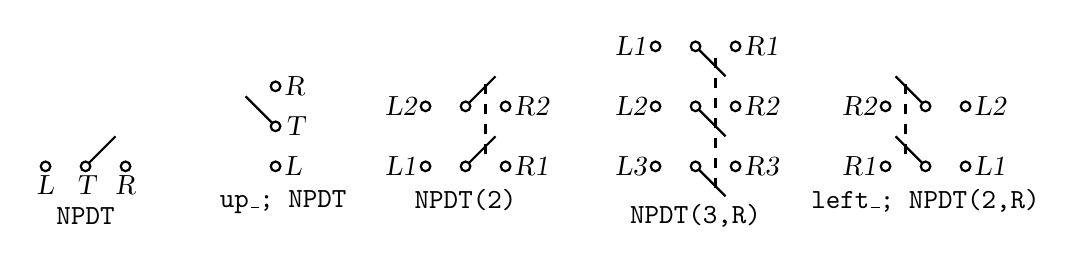
\begin{tikzpicture}[scale=2.54]
% dpic version 2020.03.01 option -g for TikZ and PGF 1.01
\ifx\dpiclw\undefined\newdimen\dpiclw\fi
\global\def\dpicdraw{\draw[line width=\dpiclw]}
\global\def\dpicstop{;}
\dpiclw=0.8bp
\dpiclw=0.8bp
\dpicdraw[fill=white](0.024,-0.061976) circle (0.009449in)\dpicstop
\dpicdraw (0.224,-0.061976)
 --(0.224,-0.061976)\dpicstop
\dpicdraw (0.224,-0.061976)
 --(0.374,0.088024)\dpicstop
\dpicdraw (0.424,-0.061976)
 --(0.424,-0.061976)\dpicstop
\dpicdraw[fill=white](0.224,-0.061976) circle (0.009449in)\dpicstop
\dpicdraw[fill=white](0.424,-0.061976) circle (0.009449in)\dpicstop
\draw (0.424,-0.085976) node[below=-2bp]{\sl R};
\draw (0.224,-0.085976) node[below=-2bp]{\sl T};
\draw (0.024,-0.085976) node[below=-2bp]{\sl L};
\draw (0.224,-0.308024) node{\tt NPDT};
\dpicdraw[fill=white](1.174,-0.061976) circle (0.009449in)\dpicstop
\dpicdraw (1.174,0.138024)
 --(1.174,0.138024)\dpicstop
\dpicdraw (1.174,0.138024)
 --(1.024,0.288024)\dpicstop
\dpicdraw (1.174,0.338024)
 --(1.174,0.338024)\dpicstop
\dpicdraw[fill=white](1.174,0.138024) circle (0.009449in)\dpicstop
\dpicdraw[fill=white](1.174,0.338024) circle (0.009449in)\dpicstop
\draw (1.198,0.338024) node[right=-2bp]{\sl R};
\draw (1.198,0.138024) node[right=-2bp]{\sl T};
\draw (1.198,-0.061976) node[right=-2bp]{\sl L};
\draw (1.212024,-0.235976) node{\tt up\_; NPDT\strut};
\dpicdraw[fill=white](1.924,-0.061976) circle (0.009449in)\dpicstop
\dpicdraw (2.124,-0.061976)
 --(2.124,-0.061976)\dpicstop
\dpicdraw (2.124,-0.061976)
 --(2.274,0.088024)\dpicstop
\dpicdraw (2.324,-0.061976)
 --(2.324,-0.061976)\dpicstop
\dpicdraw[fill=white](2.124,-0.061976) circle (0.009449in)\dpicstop
\dpicdraw[fill=white](2.324,-0.061976) circle (0.009449in)\dpicstop
\dpicdraw[fill=white](1.924,0.238024) circle (0.009449in)\dpicstop
\dpicdraw (2.124,0.238024)
 --(2.124,0.238024)\dpicstop
\dpicdraw (2.124,0.238024)
 --(2.274,0.388024)\dpicstop
\dpicdraw (2.324,0.238024)
 --(2.324,0.238024)\dpicstop
\dpicdraw[fill=white](2.124,0.238024) circle (0.009449in)\dpicstop
\dpicdraw[fill=white](2.324,0.238024) circle (0.009449in)\dpicstop
\dpicdraw[dash pattern=on 0.05in off 0.05in](2.224,-0.001976)
 --(2.224,0.373024)\dpicstop
\draw (2.348,-0.061976) node[right=-2bp]{\sl R1};
\draw (1.9,-0.061976) node[left=-2bp]{\sl L1};
\draw (2.348,0.238024) node[right=-2bp]{\sl R2};
\draw (1.9,0.238024) node[left=-2bp]{\sl L2};
\draw (2.124,-0.238024) node{\tt NPDT(2)\strut};
\dpicdraw[fill=white](3.074,0.538024) circle (0.009449in)\dpicstop
\dpicdraw (3.274,0.538024)
 --(3.274,0.538024)\dpicstop
\dpicdraw (3.274,0.538024)
 --(3.424,0.388024)\dpicstop
\dpicdraw (3.474,0.538024)
 --(3.474,0.538024)\dpicstop
\dpicdraw[fill=white](3.274,0.538024) circle (0.009449in)\dpicstop
\dpicdraw[fill=white](3.474,0.538024) circle (0.009449in)\dpicstop
\dpicdraw[fill=white](3.074,0.238024) circle (0.009449in)\dpicstop
\dpicdraw (3.274,0.238024)
 --(3.274,0.238024)\dpicstop
\dpicdraw (3.274,0.238024)
 --(3.424,0.088024)\dpicstop
\dpicdraw (3.474,0.238024)
 --(3.474,0.238024)\dpicstop
\dpicdraw[fill=white](3.274,0.238024) circle (0.009449in)\dpicstop
\dpicdraw[fill=white](3.474,0.238024) circle (0.009449in)\dpicstop
\dpicdraw[fill=white](3.074,-0.061976) circle (0.009449in)\dpicstop
\dpicdraw (3.274,-0.061976)
 --(3.274,-0.061976)\dpicstop
\dpicdraw (3.274,-0.061976)
 --(3.424,-0.211976)\dpicstop
\dpicdraw (3.474,-0.061976)
 --(3.474,-0.061976)\dpicstop
\dpicdraw[fill=white](3.274,-0.061976) circle (0.009449in)\dpicstop
\dpicdraw[fill=white](3.474,-0.061976) circle (0.009449in)\dpicstop
\dpicdraw[dash pattern=on 0.05in off 0.05in](3.374,0.478024)
 --(3.374,-0.196976)\dpicstop
\draw (3.498,0.538024) node[right=-2bp]{\sl R1};
\draw (3.05,0.538024) node[left=-2bp]{\sl L1};
\draw (3.498,0.238024) node[right=-2bp]{\sl R2};
\draw (3.05,0.238024) node[left=-2bp]{\sl L2};
\draw (3.498,-0.061976) node[right=-2bp]{\sl R3};
\draw (3.05,-0.061976) node[left=-2bp]{\sl L3};
\draw (3.274,-0.211976) node[below=-2bp]{\tt NPDT(3,R)\strut};
\dpicdraw[fill=white](4.624,-0.061976) circle (0.009449in)\dpicstop
\dpicdraw (4.424,-0.061976)
 --(4.424,-0.061976)\dpicstop
\dpicdraw (4.424,-0.061976)
 --(4.274,0.088024)\dpicstop
\dpicdraw (4.224,-0.061976)
 --(4.224,-0.061976)\dpicstop
\dpicdraw[fill=white](4.424,-0.061976) circle (0.009449in)\dpicstop
\dpicdraw[fill=white](4.224,-0.061976) circle (0.009449in)\dpicstop
\dpicdraw[fill=white](4.624,0.238024) circle (0.009449in)\dpicstop
\dpicdraw (4.424,0.238024)
 --(4.424,0.238024)\dpicstop
\dpicdraw (4.424,0.238024)
 --(4.274,0.388024)\dpicstop
\dpicdraw (4.224,0.238024)
 --(4.224,0.238024)\dpicstop
\dpicdraw[fill=white](4.424,0.238024) circle (0.009449in)\dpicstop
\dpicdraw[fill=white](4.224,0.238024) circle (0.009449in)\dpicstop
\dpicdraw[dash pattern=on 0.05in off 0.05in](4.324,-0.001976)
 --(4.324,0.373024)\dpicstop
\draw (4.2,-0.061976) node[left=-2bp]{\sl R1};
\draw (4.648,-0.061976) node[right=-2bp]{\sl L1};
\draw (4.2,0.238024) node[left=-2bp]{\sl R2};
\draw (4.648,0.238024) node[right=-2bp]{\sl L2};
\draw (4.424,-0.238024) node{\tt left\_; NPDT(2,R)\strut};
\end{tikzpicture}
\vspace*{-0.5\baselineskip}
